\begin{figure}[h]
    \centering
    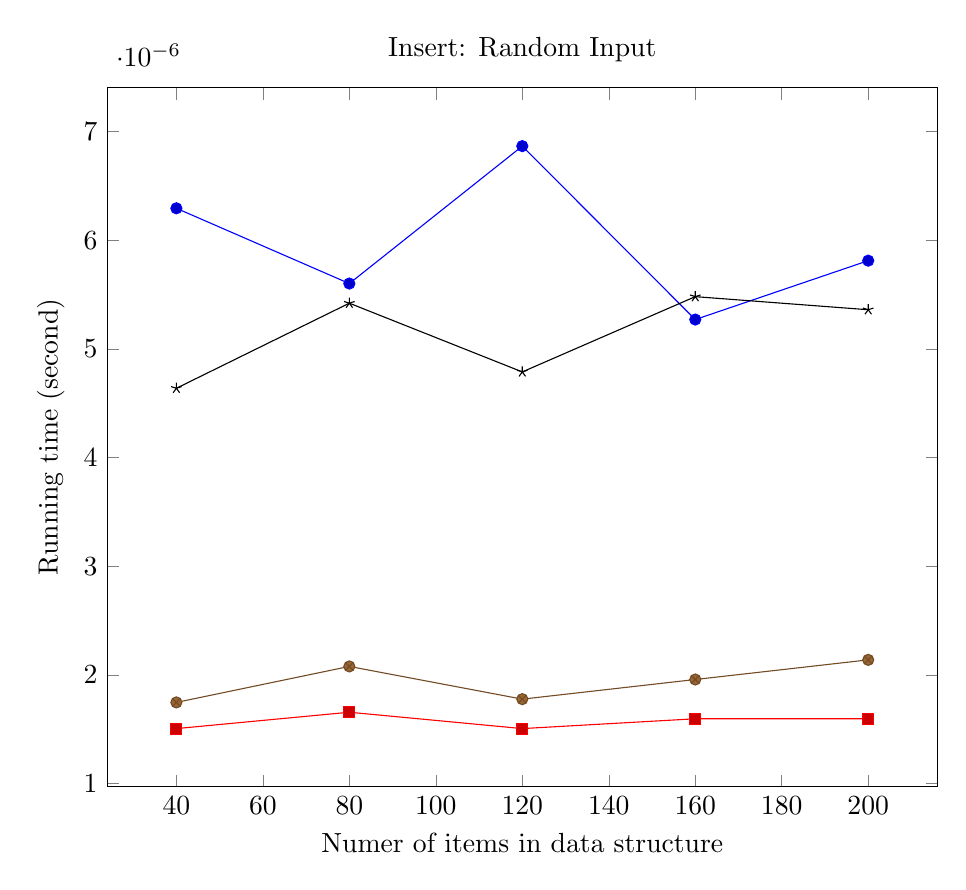
\begin{tikzpicture}
        \begin{axis}[
            xlabel={Numer of items in data structure},
            ylabel={Running time (second)},
            title={Insert: Random Input},
            width=\textwidth
        ]
		\addplot coordinates {
			(40, 6.2945645381090595e-06)
			(80, 5.601861263579422e-06)
			(120, 6.866797677937409e-06)
			(160, 5.270568393153652e-06)
			(200, 5.812683999306678e-06)
		};
		\addplot coordinates {
			(40, 1.5058766837577896e-06)
			(80, 1.6564643521344013e-06)
			(120, 1.5058766837577896e-06)
			(160, 1.5962292847837566e-06)
			(200, 1.5962292847837566e-06)
		};
		\addplot coordinates {
			(40, 1.7468169531603683e-06)
			(80, 2.0781098235861386e-06)
			(120, 1.7769344868356906e-06)
			(160, 1.9576396888848492e-06)
			(200, 2.138344890936783e-06)
		};
		\addplot coordinates {
			(40, 4.638100185974659e-06)
			(80, 5.421156061527488e-06)
			(120, 4.78868785435127e-06)
			(160, 5.481391128878132e-06)
			(200, 5.360920994179619e-06)
		};
        \legend{}
        \end{axis}
    \end{tikzpicture}
    \caption{Average of 0 operations, benchmarked every 0, starting at 0.}
\end{figure}